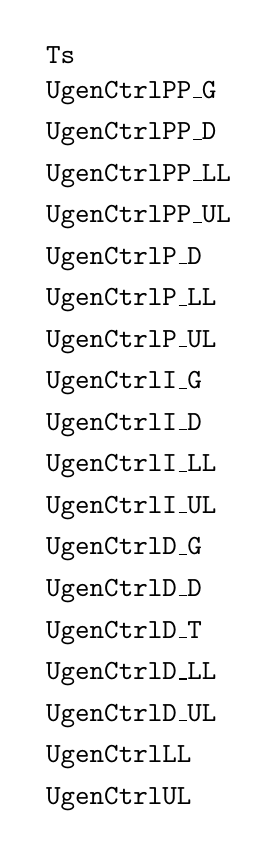
\begin{tikzpicture}[node distance=.5cm]
    \begin{scope}[]
    	    \matrix[column 1/.style={anchor=base west}]{
             \node[] {\texttt{Ts}}; \\
             \node[] {\texttt{UgenCtrlPP\_G}}; \\
             \node[] {\texttt{UgenCtrlPP\_D}}; \\
             \node[] {\texttt{UgenCtrlPP\_LL}}; \\
             \node[] {\texttt{UgenCtrlPP\_UL}}; \\
             \node[] {\texttt{UgenCtrlP\_D}}; \\
             \node[] {\texttt{UgenCtrlP\_LL}}; \\
             \node[] {\texttt{UgenCtrlP\_UL}}; \\
             \node[] {\texttt{UgenCtrlI\_G}}; \\
             \node[] {\texttt{UgenCtrlI\_D}}; \\
             \node[] {\texttt{UgenCtrlI\_LL}}; \\
             \node[] {\texttt{UgenCtrlI\_UL}}; \\
             \node[] {\texttt{UgenCtrlD\_G}}; \\
             \node[] {\texttt{UgenCtrlD\_D}}; \\
             \node[] {\texttt{UgenCtrlD\_T}}; \\
             \node[] {\texttt{UgenCtrlD\_LL}}; \\
             \node[] {\texttt{UgenCtrlD\_UL}}; \\
             \node[] {\texttt{UgenCtrlLL}}; \\
             \node[] {\texttt{UgenCtrlUL}}; \\
        };
    \end{scope}
\end{tikzpicture}